\section[Witnessing metrologically useful entanglement]
{Witnessing metrologically useful {\color{grey} X} entanglement}
\thiswatermark{\put(1,-282){\color{l-grey}\rule{84pt}{88pt}}
\put(84,-282){\color{grey}\rule{410pt}{88pt}}}


\quotes{Adrien-Marie Legendre}{All the truths of mathematics are linked to each other,

and all means of discovering them are equally admissible.}

\lettrine[lines=2, findent=3pt,nindent=0pt]{T}{ypically}, one has not access to the density matrix of the system been used for metrology or for other quantum process.
Moreover, for systems on which the particle number is very large, this is the case when one wants to do metrology with quantum states, the details of the density matrix are forbidden by practical reasons.
Since the quantum Fisher information is based on the complete knowledge of the density matrix, shortcuts to avoid the complete tomography must be developed as we have had shown one practical case on the previous chapter.
In this chapter, we obtain a general procedure to get an optimal bound for the quantum Fisher information based on as many expectation values of the initial state as one is ready to measure.
Two main features are worth to mention again.
First, in general this method gives us an optimal tight bound.
Last but not least, the bound is based on the expectation values of the initial state only, so it is not necessary to perform an evolution of the state to estimate how well will it behave.
This is in contrast to other approaches one can find in the literature, an it is a time saving concept.

The figure of merit of bounds from below for the quantum Fisher information based on expectation values of the initial state is the following,
\be
  \qfi [\rho,J_z] \geq \frac{\expect{J_x}^2}{\varian{J_y}}.
\ee
where the state is polarized along the $x$-axis and the variance of the $J_y$ operator is smaller than the standard.
On the previous chapter we also have shown one of these bound specifically designed for unpolarized Dicke states.

Homogeneous magnetometry, $\bs{B} = B\bs{k}$ where $B$ is constant in time.

Section~[REF], see magnetometry, generator $J_z$.

Quantum Fisher information $\qfi [\rho, J_z]$.

\subsection{Bound from below of a function convex over the states given some arbitrary expectation values}

The problem of getting a lower bound for a convex function on the states having already some expectation values of some arbitrary observables was studied by O. G\"uhne {\it et al.} and J. Eisert {\it et al.} in Refs.~\citep{Guehne2007, Eisert2007} respectively, mainly from the perspective of entanglement measures.
The illustrated techniques are based on the well known Legendre transform for differentiable functions, see Appedix~\ref{app:legendre-transform} for more details.
We first review in this section the state-of-the-art solution for this problem.
And later on, we extend it to the quantum Fisher information.
For simplicity in the next subsection, Sec~\ref{}, we assume that a single expectation value is given.
An extension to the case on which more expectation values are given will follow in the Subsection~\ref{}.
Finally, we will summarize it with an explicit formula which will be used to compute the bounds.

\subsubsection{Estimation of a general convex function based on the expectation value of an arbitrary observable}

When a convex function $g(\rho)$ is given together with an expectation value of some operator $w=\tr(\rho W)$, a tight lower bound can be obtained as \citep{Rockafellar1996, Guehne2007, Eisert2007}
\be
  \label{eq:lt-lower-bound-single-parameter}
  \begin{split}
    g(\rho)\geq\mathcal{B}_g(w):=\,&\sup_r \{ rw - \hat{g}(rW)\}\\
    =\,& \{\min_{\rho}g(\rho)|w = \tr(\rho W)\}
  \end{split}
\ee
where $\hat{g}(rW)$ is the Legendre transform of $g(\rho)$ and the second inequality refers only to the tightness of our bound.
The Legendre transform in this context is defined as
\be
  \label{eq:lt-for-convex-function-single-parameter}
  \hat{g}(rW)=\sup_{\rho}\{\expect{rW}_\rho - g(\rho)\}.
\ee
This method has been used to compute entanglement measures, as we mentioned before.

Following the theory one can find that in the case on which the convex function $g(\rho)$ is defined as convex roof over all possible convex decompositions of the state, the optimisation of Eq.~(\ref{eq:lt-for-convex-function-single-parameter}) can be reduced to an optimisation over pure states only, thus simplifying the process \cite{}.
However, even an optimization over all pure states is feasible numerically only for small systems.
We will show later on this section circumvent this issue in the case of the QFI.
The convex construction has the following form
\be
  g(\rho) = \inf_{\{p_k,\psi_k\}} \sum_{k}p_k g(\ket{\psi_k}),
\ee
where the mixed state is decomposed into $\rho = \sum_k p_k \ketbra{\psi_k}{\psi_k}$.
We notice in our approach that the QFI is the convex roof of $4\varian{J_z}$ as it was shown on Ref.~\citep{Toth2007}.
Hence, we will be able to use this simplification to apply this method to obtain the lower bound on the QFI.

For this purpose we simplify our discourse to one expectation value and therefore one observable, $w = \tr(\rho W)$.
Later we will extend our results to the multi-parameter case.

Notice that the tightest bound from below on of such a function $g(\rho)$ is convex too on the expectation values\ie $\mathcal{B}_g(w)$ is convex if $g(\rho)$ is convex.
This is shown in the following way,

Therefore, theory tells us that we can use the Legendre transform to get rid of the state preserving all the necessary information to reconstruct the $\mathcal{B}_{g}$ bound from the expectation values, this can be found on the work of Prof.~G\"uhne and Prof.~Werner Reference~\citep{} and for a brief description of the properties of the Legendre transform see Appendix~\ref{ap:}.
In this case the Legendre transform can be written in the following way,
\be
  \hat{g}(rW) = \sup_{\rho}\{ r\expect{W}_{\rho}-g(\rho)\}.
\ee

Now we have the Legendre transform, we recover the bound from below of $g(\rho)$ as
\be
  \label{eq:lt-generic-bound-for-convex-func}
  \mathcal{B}_g (w) = \sup_{r}\big\{rw-\sup_{\rho}\{r\expect{W}_{\rho}-g(\rho)\}\big\}.
\ee
To clarify, notice that the $\rho$ appearing on the inner maximization is not related with the one appearing on $g(\rho)$ that is bounded by $\mathcal{B}_g$ but a variable state for the maximization.

The Equation~(\ref{eq:lt-generic-bound-for-convex-func}) has been applied on entanglement measures, when $g(\rho)$ is defined using the convex roof construction\ie the function $g(\rho)$ is extended from the well defined region, namely the region of pure states, to the mixed states using the convex roof construction.
For illustrative purposes the convex roof of a function defined for pure states is the following,
\be
  g(\rho) = \inf_{\{p_k,\ket{\phi_k}\}}\big\{\sum_{k}p_k g(\ket{\phi_k})\big\}
\ee
for any decomposition $\rho=\sum_k p_k \ketbra{\phi_k}{\phi_k}$
In this case the Equation~(\ref{eq:lt-generic-bound-for-convex-func}) can be further simplified.
Let us focus by now on the inner maximization,
\be
\begin{split}
  \hat{g}(rW) & = \sup_{\rho}\{r\expect{W}_\rho - g(\rho)\} \\
  &=\sup_{\rho}\Big\{r\expect{W}_\rho - \inf_{\{p_k,\ket{\phi_k}\}}\big\{\sum_{k} p_k g(\ket{\phi_k})\big\} \Big\} \\
  &=\sup_{\{p_k, \ket{\phi_k}\}} \Big\{ \sum_k p_k r\expect{W}_{\ket{\phi_k}} - \inf_{\{p_k, \ket{\phi_k}\}} \big\{\sum_k p_k g(\ket{\phi_k}) \big\}  \Big\} \\
  &=\sup_{\{p_k, \ket{\phi_k}\}} \Big\{ \sum_k p_k \big\{ r\expect{W}_{\ket{\phi_k}} - g(\ket{\phi_k}) \big\} \Big\} \\
  &=\sup_{\ket{\psi}} \big\{ r\expect{W}_{\ket{\psi}} - g(\ket{\psi}) \big\}.
\end{split}
\ee
So now we have restricted the maximization to only pure states as it is shown on Reference~\citep{}.

One the other hand, one can find different definitions of the QFI in the literature.
Among those definitions, there is one that defines the QFI as the convex roof of four times the variance of the generator of the unitary phase shift that suffers the state \citep{}.
This can be written in the following way,
\be
  \qfi[\rho, G] = \inf_{\{p_k, \ket{\phi_k}\}}4\sum_k p_k (\Delta G)_{\ket{\phi_k}}^2
\ee

Even further simplification can be achieved for quantum Fisher information,
\be
\begin{split}
  \hat{\qfi}(rW) &= \sup_{\ket{\psi}}\big\{r\expect{W}_{\ket{\psi}}-4\varian{J_z}_{\ket{\psi}}\big\} \\
  &= \sup_{\ket{\psi}} \big\{ r\expect{W}_{\ket{\psi}}-4\expect{J_z^2}_{\ket{\psi}} + 4\expect{J_z}^2_{\ket{\psi}} \big\} \\
  &= \sup_{\ket{\psi}} \{\expect{rW-4J_z^2}_{\ket{\psi}} +
  \expect{2J_z}^2_{\ket{\psi}}\},
\end{split}
\label{eq:lt-legendre-of-qfi}
\ee
which is clearly a second order maximization over pure states.

With that at hand we are able to prove the following observation: the Legendre transform of the highest lower bound of the quantum Fisher information when the expectation value of some operator $W$ is known, can be written as the maximization over some parameter $\mu$ of the highest eigenvalue  $\lambda_{\max}(rW-4(J_z-\mu)^2)$.
This can  be expressed as follows,
\be
  \hat{\qfi}(rW) = \sup_\mu \{\lambda_{\max} (rW-4(J_z-\mu)^2)\},
\ee
where at the maximum the derivative with respect to $\mu$ must be zero for this quadratic function on the state.
Hence, the value of $\mu$ will coincide with the expectation value on the optimal state $\expect{J_z}_{\psi}$
Therefore, the finding of the optimal parameter $\mu$ is delimited to the range defined by $[\expect{J_z}_{\min},\expect{J_z}_{\max}]$.
For qubits this means that we have to perform a search for $\mu_{\text{opt}}$ in between $-N/2\leq \mu \leq N/2$.

Another way of getting the result of the maximization for the second order equation is parameterizing the eigenstate with the maximum eigenvalue of the operator $rW-4(J_z-\mu)^2$, so we get $\ket{\phi_{\max}(\mu)}$, and finally computing the expectation values of Equation~(\ref{eq:lt-legendre-of-qfi}) and maximizing it.

With this a tight bound from below for the quantum Fisher information can be found when the expectation value of an observable, say $W$, is known as follows,
\be
  \mathcal{B}_{\mathcal{F}}(w) = \sup_r \big\{ rw - \sup_{\ket{\psi}} \{\expect{rW-4J_z^2} + \expect{2J_z}^2\}\big\}.
\ee
One may notice that the inner maximization is a second order maximization.

\subsubsection{Measuring several observables}

Which is the lowest possible value of $g(\rho)$ for a state where some expectation values of $\{W_{i}\}_{i=1}^M$ operators, $w_i = \tr(\rho {W}_i)$ are known?

Such bound is defined in a way to fulfill the following inequality,
\be
  g(\rho) \geq \mathcal{B}_{g}(w_1,w_2,...) := \big\{\min_{\rho}g(\rho) \,|\,  \{w_i = \tr(\rho {W}_i)\}_{i=1}^M\big\}.
\ee
When computing this bound we will require to this to be as tight as possible.

This can be extended for several observables as follows
\be
  \mathcal{B}_{\mathcal{F}}(w_1,w_2,...) = \sup_{\bs{r}} \big\{ \bs{rw} - \sup_{\ket{\psi}} \{\expect{\bs{rW}-4J_z^2} + \expect{2J_z}^2\}\big\},
\ee
where $\bs{r}=(r_1,\dots,r_m)$ is the vector form and the same applies to $\bs{w}$ and the operators set $\bs{W}$.
The contraction of two of those vectors must be seen as a scalar product\ie $\bs{rW}=\sum r_iW_i$ where $W_i$ is the corresponding $i^{\text{th}}$ operator of $\bs{W}$.

\begin{figure}
  \centering
  \igwithlabel{(a)}{scale=.65}{img/plots/LT_fidGHZ.pdf}
  \igwithlabel{(b)}{scale=.65}{img/plots/LT_fidDicke.pdf}
  \caption{(a) Analytical solution of the bound $\mathcal{B}_{\mathcal{F}}$ for different values of the fidelity with respect to the GHZ state. (b) Numerical results for the minimum quantum Fisher information as a function of the fidelity with respect of unpolarise Dicke states perpendicular to the magnetic field, $|\text{D}_N^0\rangle$. (blue-line) For systems with 4 particles and (red-dashed) for system with 8 particles. One may notice that when the fidelity is at its maximum the bound approaches to 0.5 as it is the quantum Fisher information for large particle number.}
  \label{fig:vd-secuence-evo}
\end{figure}

\begin{figure}
  \centering
  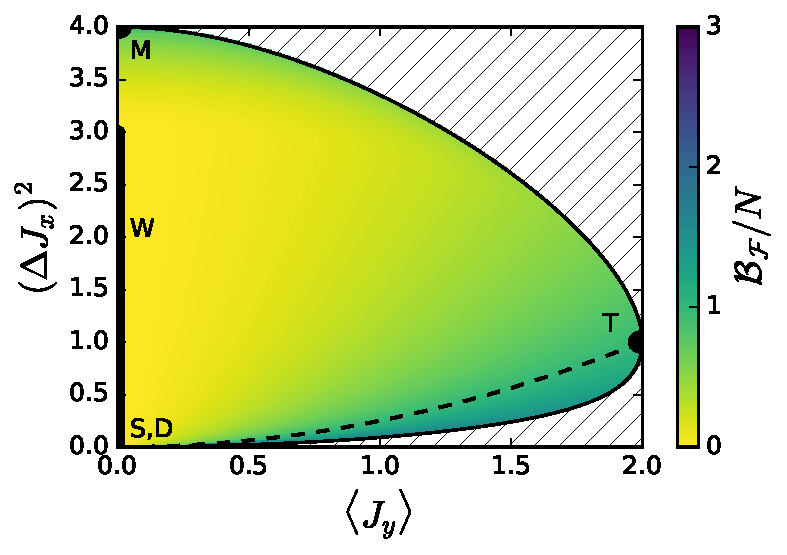
\includegraphics[scale=.65]{img/plots/LT_spsq2d_4.pdf}
  \caption{We show as a function of the expectation value, $\expect{J_y}$, and the variance in the perpendicular direction, $\varian{J_x}$, the minimum sensitivity for a 4-qubit system.
  (hatched) The physically forbidden region is indicated. (M,T,S,D) Those points indicate where the mixed state (), the totally polarized state (), the single state and the unpolarized Dicke state would be located. (W) on this line sit any of the states which is a mixture between the completely mixed state of the symmetric subspace and the singlet state among others, for instance the completely mixed state of the whole Hilbert space. (dashed) It indicates the shot-noise threshold where below it non-classical sensitivities can be achieved.}
  \label{fig:lt-spsq2d-4}
\end{figure}

\begin{figure}
  \centering
  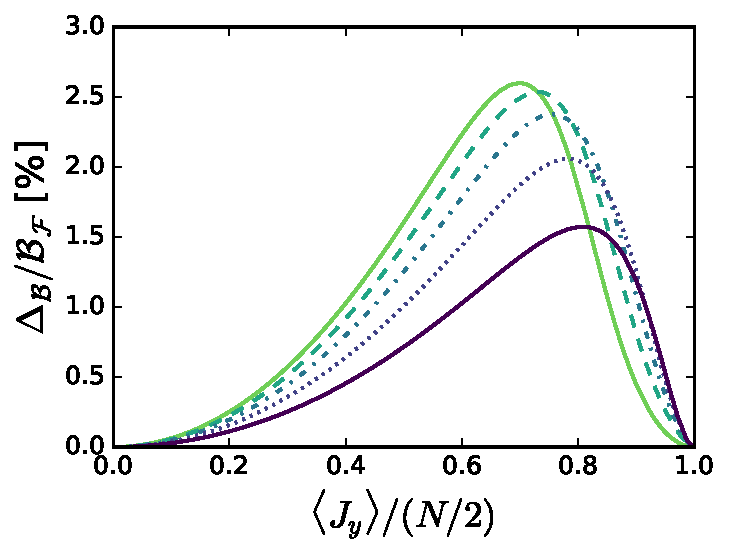
\includegraphics[scale=.65]{img/plots/LT_edge_diff.pdf}
  \caption{Difference between the bound of Pezze-Smerzi and the optimal bound for the quantum Fisher information normalized by the value of the optimal bound itself for the bosonic ground states of $H=J_x^2-\lambda J_y$ for $\forall \lambda \in [0,\infty)$.
  From dark to lighter colors (line, point, dash-point, dashed, pointed, line), results for different particle numbers, $N=4,6,10,20,1000$ respectively.
  Heuristically speaking, one can say that for large particle number the difference is biggest when the polarisation is around two thirds of the maximal polarisation and that this difference is about $2.6\%$.}
  \label{fig:lt-edge-diff}
\end{figure}

\begin{figure}
  \centering
  \igwithlabel{(a)}{scale=.65}{img/plots/LT_spsq_scaling_1.pdf}
  \igwithlabel{(b)}{scale=.65}{img/plots/LT_spsq_scaling_2.pdf}
  \caption{}
  \label{fig:lt-spsq-scaling}
\end{figure}

\begin{figure}
  \centering
  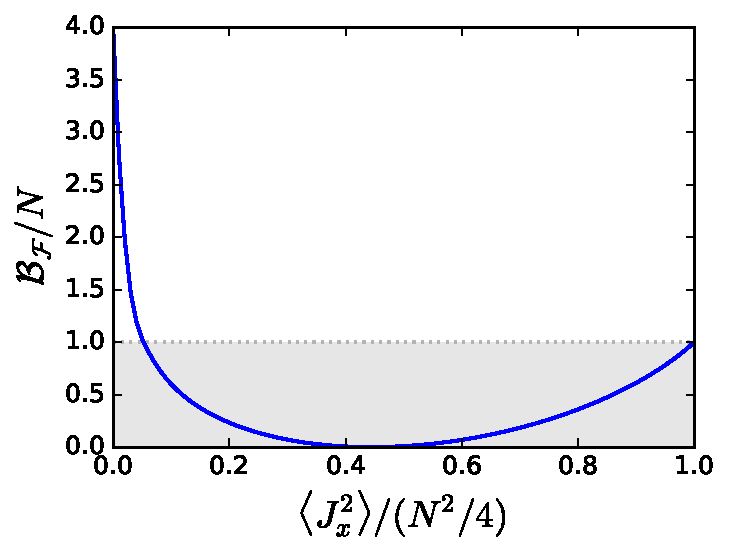
\includegraphics[scale=.65]{img/plots/LT_dicke_edge.pdf}
  \caption{The numerics shows us a tiny region the symmetric system surpassing the shot-noise threshold.}
  \label{fig:vd-secuence-evo}
\end{figure}

\begin{figure}
  \centering
  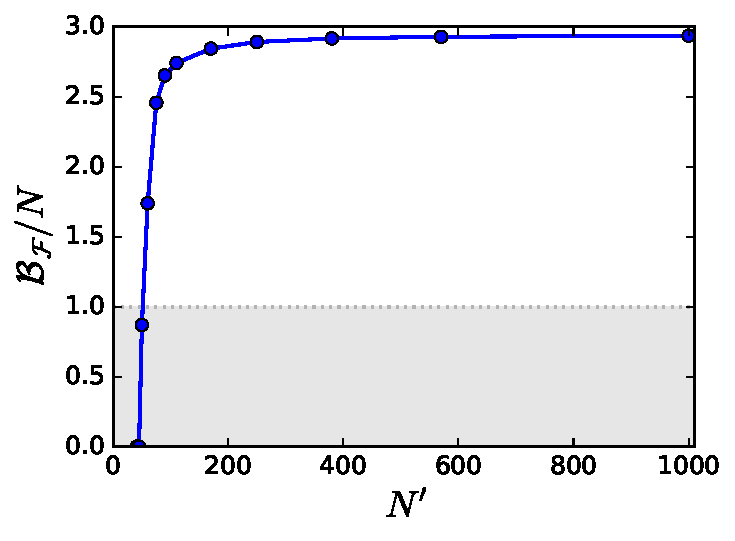
\includegraphics[scale=.65]{img/plots/LT_dicke_7900_asymp.pdf}
  \caption{Secuence of the evolution of an unpolarized Dicke state of 16 qubits for $\Theta=\{i\pi/6\}_{i=0}^4$. Bloch spheres representing the Hirusi distribution of the state, and below PDF of the $J_x$ POVM for each step of the secuence}
  \label{fig:vd-secuence-evo}
\end{figure}
